\section {Conclusions}

% intro-type paragraph here
The aqueous chemistry taking place in the Earth's atmosphere is governed by the physics and chemistry of the water surfaces found there. Many recent experiments have revealed specific pathways for reaction of \suldiox, but the molecular-level nature of those reactions are still poorly understood. Through computer simulations we are able to probe the microscopic environments in which those reactions occur, and better understand the conditions in which \suldiox~reacts.

We have presented the results of several classical simulations of \suldiox~interacting with an aqueous surface. We set out to find the orientational behavior of \wat~and \suldiox~through depth-profiling of molecular orientational distributions. In previous experimental studies we posited that water reorients in the presence of \suldiox, and this behavior is one of the steps in formation of gaseous hydrate complexes on water's surface. Spectroscopic techniques can not precisely define a depth profile or orientational distribution of adsorbed species, so we have used molecular dynamics simulations to gain that information.

Our simulations recreated the experimental setup of a recent study by our group,\cite{Ota2011} by introducing a concentrated gas phase of \suldiox~to a water surface. Through simulation it was found that gaseous \suldiox~quickly adsorbs to the water surface, and continues to bind until a complete surface coverage is reached. Surface waters reorient in the presence of adsorbed \suldiox. The waters at the interface of a neat-water surface tend to lay flatter to the surface than when a saturating layer of \suldiox~is present. The waters interacting with the layer of adsorbed \suldiox~orient more perpendicularly to the interface, and further expose their ``free-OH'' uncoupled bonds for interactions with \suldiox, and hydrate complex formation. Furthermore, we have found that surface waters underneath a blanket layer of adsorbed \suldiox~will penetrate further into the gas phase, allowing for greater mobility of waters away from the aqueous bulk.

The surface behavior of the \suldiox~molecules was also determined, information that is difficult to obtain with vibrational sum-frequency spectroscopy. Through these simulations we are able to characterize the orientational behavior of \suldiox~during and after adsorption. Our equilibrium simulations show that a single \suldiox~molecule, representing a low concentration, has a high surface affinity. At a high \suldiox~concentration, unreacted \suldiox~molecules are found further out of the water phase as a bound layer of \suldiox~crowds the surface and binds all the surface waters. The orientation of \suldiox~on the water surface was found to be similar for both low and high concentrations. Those \suldiox~molecules at or below the surface strongly orient with the sulfur atom pointed in towards the water bulk, and the oxygen atoms out towards the gas phase. The \suldiox~slightly above the water surface loses the orientational preference within 10 $\AA$ and those further from the water are more isotropically oriented. Figure \ref{fig:so2-surface-cartoon} depicts what the neat-water and saturated surfaces might look like for both \suldiox~and \wat~orientations and locations.

\begin{figure}[h!]
	\begin{center}
		\includegraphics[scale=1.0]{images/angle-cartoons/system-surface.png}
		\caption{\wat~and \suldiox~both exhibit preferred orientations in the region near the liquid-gas interface. The neat-water system (A) with a single \suldiox~molecule (low-concentration) has surface waters orienting mostly flat to the interface. When the \suldiox~concentration is increased, as in the saturated system (B), the waters at the surface behave similar to the neat-water interface, but waters that venture into the adsorbed \suldiox~gas layer orient strongly with their bisectors pointing out from the aqueous phase towards the gas. In both cases, the \suldiox~orients with its molecular bisector pointing out to the gas phase when it is near the surface.}
		\label{fig:so2-surface-cartoon}
	\end{center}
\end{figure}

Steered molecular dynamics simulations were used to model the behavior of an adsorbing \suldiox~as it moves from the gas phase above the water down through the surface and into the bulk. The results for the transit through the interface show that in both systems of low and high \suldiox~concentration an adsorbing \suldiox~has very similar orientation to those already bound to the water surface. The \suldiox~reorients as it makes its first contact with the water surface. Within 5 $\AA$ of the surface the \suldiox~is mostly oriented with its sulfur towards the water phase. The \suldiox~pulled further into the water bulk retains its orientation until it is past the interfacial region and then isotropically orients with the bulk water.

Having now examined this passageway of \suldiox~from the gas to adsorbed aqueous phases, we may turn to further filling in the details of adsorption and interfacial chemistry of gas molecules. What species form during the adsorption transition, and how do molecular properties affect the process? Can we form a theory that will more fully explain the transit of many small molecules of environmental and industrial interest? This study is one of several aiming to characterize \suldiox~adsorption and behavior on aqueous surfaces. We plan to report further results of ongoing computational simulation and experimental studies regarding temperature and chemical constituent effects on atmospherically relevant water surfaces.
